\documentclass[journal,dvipsnames]{acmart}

% ── Metadata ──────────────────────────────────────────────────────────
\acmJournal{TIST}
\acmVolume{1}
\acmNumber{1}
\acmArticle{1}
\acmYear{2026}
%\acmDOI{10.1145/3589307}

% ── Packages ──────────────────────────────────────────────────────────
\usepackage[utf8]{inputenc}
\usepackage[T1]{fontenc}
\usepackage{booktabs}
\usepackage{enumitem}
\usepackage{graphicx}
\usepackage{tikz}
\usetikzlibrary{arrows.meta,positioning,fit}
\usepackage{caption}
\usepackage{listings}
\usepackage{float}
\usepackage{microtype}

% ── Listing Configuration for YAML ─────────────────────────────
\lstdefinelanguage{YAML}{
  sensitive=false,
  comment=[l]{\#},
  morecomment=[s]{/*}{*/},
  morestring=[b]",
  morestring=[b]',
  morekeywords={true,false,null,yes,no,on,off},
  keywordstyle=\color{teal!60!black}\bfseries,
  commentstyle=\color{gray!70!black}\itshape,
  stringstyle=\color{violet!65!black},
}

\lstset{
  language=YAML,
  basicstyle=\small\ttfamily,
  backgroundcolor=\color{black!1},
  emph={id,version,model,provider,name,parameters,embedding,system_prompt,planning_prompt,query_analyzer_prompt,tools,definitions,flow,strategy,max_turns,key_events,description,num_users,duration_days,company_name,industry,company_size,user_id,query,assertions,entity_list,entity_type,entity_id,prompts,citation_relevance,assertion_check,score,explanation,final_score,summary},
  emphstyle=\color{blue!65!black}\bfseries,
  breaklines=true,
  columns=fullflexible,
  keepspaces=true,
  showstringspaces=false,
  xleftmargin=8pt,
  xrightmargin=8pt,
  framexleftmargin=5pt,
  frame=tb,
  rulecolor=\color{black!20},
  framerule=0.5pt,
  aboveskip=8pt,
  belowskip=8pt,
  captionpos=b,
  numbers=left,
  numberstyle=\tiny\color{gray},
  numbersep=5pt,
  literate=
    {á}{{\'a}}1 {é}{{\'e}}1 {í}{{\'i}}1 {ó}{{\'o}}1 {ú}{{\'u}}1
    {Á}{{\'A}}1 {É}{{\'E}}1 {Í}{{\'I}}1 {Ó}{{\'O}}1 {Ú}{{\'U}}1
    {à}{{\`a}}1 {è}{{\`e}}1 {ì}{{\`i}}1 {ò}{{\`o}}1 {ù}{{\`u}}1
    {À}{{\`A}}1 {È}{{\'E}}1 {Ì}{{\`I}}1 {Ò}{{\`O}}1 {Ù}{{\`U}}1
    {ä}{{\"a}}1 {ë}{{\"e}}1 {ï}{{\"i}}1 {ö}{{\"o}}1 {ü}{{\"u}}1
    {Ä}{{\"A}}1 {Ë}{{\"E}}1 {Ï}{{\"I}}1 {Ö}{{\"O}}1 {Ü}{{\"U}}1
    {â}{{\^a}}1 {ê}{{\^e}}1 {î}{{\^i}}1 {ô}{{\^o}}1 {û}{{\^u}}1
    {Â}{{\^A}}1 {Ê}{{\^E}}1 {Î}{{\^I}}1 {Ô}{{\^O}}1 {Û}{{\^U}}1
    {œ}{{\oe}}1 {Œ}{{\OE}}1 {æ}{{\ae}}1 {Æ}{{\AE}}1 {ß}{{\ss}}1
    {ç}{{\c c}}1 {Ç}{{\c C}}1 {ø}{{\o}}1 {Ø}{{\O}}1 {å}{{\r a}}1 {Å}{{\r A}}1
    {€}{{\euro}}1 {£}{{\pounds}}1 {«}{{\guillemotleft}}1
    {»}{{\guillemotright}}1 {ñ}{{\~n}}1 {Ñ}{{\~N}}1 {¿}{{?`}}1
    {-}{{-}}1
}

% ── Title and Author ─────────────────────────────────────────────────────
\title{EABench: A Configurable Benchmark Framework for Evaluating LLM-Powered Enterprise Agents}

\author{Haoyi Xiong}
\affiliation{%
  \institution{Microsoft Corporation}
  \city{Beijing}
  \country{China}
}
\author{Yi Liu}
\affiliation{%
  \institution{Microsoft Corporation}
  \city{Beijing}
  \country{China}
}
\author{Bin Zhu}
\affiliation{%
  \institution{Microsoft Corporation}
  \city{Beijing}
  \country{China}
}
\author{Zhongxian Jia}
\affiliation{%
  \institution{Microsoft Corporation}
  \city{Beijing}
  \country{China}
}
\author{Yiqin Yu}
\affiliation{%
  \institution{Microsoft Corporation}
  \city{Beijing}
  \country{China}
}
\author{Yi Wang}
\affiliation{%
  \institution{Microsoft Corporation}
  \city{Beijing}
  \country{China}
}

\begin{abstract}
Large language model (LLM) agents are increasingly deployed in enterprise
productivity settings---automatically managing emails, scheduling meetings,
retrieving files, and executing multi-step workflows across heterogeneous data
sources.  Despite rapid progress in general-purpose agent benchmarks, existing
evaluation frameworks fall short in two important respects: they provide little
support for generating \emph{realistic enterprise data at scale}, and they
offer limited flexibility in \emph{agent architecture configuration}.  We
present \textbf{EABench}, namely \emph{\underline{E}nterprise \underline{A}gentics 
\underline{Bench}mark}, an open-source benchmark framework designed to
address both gaps.  EABench provides (1)~an LLM-driven \emph{synthetic data
generation} pipeline that produces coherent, inter-connected corporate corpora
spanning emails, meetings, files, chats, and channels; (2)~a
\emph{configurable agent runtime} that supports multiple execution strategies
(ReAct and Plan-and-Execute) and multiple LLM backends through a
provider-agnostic interface; (3)~a comprehensive \emph{enterprise tool suite}
encompassing semantic search over all content types, sandboxed file I/O, and
code execution; and (4)~a \emph{multi-dimensional evaluation harness} combining
deterministic assertions, citation relevance scoring, and LLM-as-a-Judge for
end-to-end and user-level evaluation.  Together, these components enable
systematic, reproducible comparison of agent designs under realistic enterprise
conditions.
\end{abstract}

\ccsdesc[500]{Computing methodologies~Artificial intelligence}
\ccsdesc[500]{Computing methodologies~Machine learning}

\keywords{LLM agents, enterprise AI, benchmarking, evaluation frameworks, synthetic data generation}

\begin{document}

\maketitle

% ══════════════════════════════════════════════════════════════════════
% 1  INTRODUCTION
% ══════════════════════════════════════════════════════════════════════
\section{Introduction}
\label{sec:intro}

The emergence of LLM-based autonomous agents capable of using tools, planning multi-step workflows, and interacting with external APIs has prompted a wave of benchmarks aimed at measuring agent capability. However, enterprise environments represent the ultimate frontier for agentic deployment, characterized by a unique and convergence of operational constraints. Enterprise AI agents must navigate immense, \emph{heterogeneous} corpora---email threads, calendar invites, document repositories, instant messages, and project channels---where information is \emph{fragmented} across diverse data silos, strictly \emph{access-controlled} at the user level, and \emph{temporally distributed} across weeks or months of complex organizational history.

Current benchmarks such as WebArena~\cite{zhou2023webarena},
AgentBench~\cite{liu2023agentbench}, ToolBench~\cite{qin2023toolllm}, and recently
proposed advanced evaluations like GAIA-2~\cite{gaia2} focus primarily on web navigation,
software engineering tasks, generic API calling, and complex multimodal reasoning.
While these settings surface important general capabilities, they suffer
from critical structural limitations. First, they rely almost entirely on
static, pre-computed datasets, providing no inherent mechanisms for users
to generate novel, domain-specific data. Second, they severely lack
configurability, often locking researchers into rigid agent designs that
prevent fine-grained ablation studies. Consequently, they fail to capture the
\emph{enterprise information retrieval and synthesis} tasks that constitute
the bulk of knowledge-worker workloads---such as prioritizing action items
from incident post-mortems or securely tracing contract negotiations. Perhaps
most importantly, this lack of configurability and dynamic data generation
stifles opportunities for the open-source community: applied sciences require
flexible sandboxes to systematically investigate, diagnose, and tailor
agentic architectures and workflows.

Consider an applied researcher aiming to evaluate whether a novel memory module improves an agent's ability to summarize a 30-day project. Current benchmarks offer no way to dynamically generate that 30-day organizational timeline, nor do they provide a standardized mechanism to securely plug the novel memory module into the agentic workflow. EABench directly targets this gap by reimagining benchmarking as an \textbf{open-source experimental sandbox}. Rather than simply measuring performance against fixed tasks, EABench democratizes agent architecture research through extreme generative scale and a fully parameterized configuration-as-code design. Table~\ref{tab:comparison} summarizes how EABench compares with existing
benchmarks across key dimensions.

\begin{table*}[t]
\centering
\caption{Comparison of EABench with existing agent benchmarks: DRBench~\cite{abaskohi2025drbench}, HERB~\cite{choubey2025benchmarking}, and others. $\checkmark$ = supported, Partial = partially supported, -- = not supported.}
\label{tab:comparison}
\small
\begin{tabular}{lcccccc c}
\toprule
\textbf{Feature} & \textbf{WebArena} & \textbf{AgentBench} & \textbf{ToolBench} & \textbf{WorkArena} & \textbf{DRBench} & \textbf{HERB} & \textbf{EABench} \\
\midrule
Multi-source enterprise data          & --            & --             & --             & Partial        & $\checkmark$   & $\checkmark$   & $\checkmark$ \\
Synthetic data generation             & --            & --             & --             & --             & Partial        & $\checkmark$   & $\checkmark$ \\
Configurable agent strategies         & --            & --             & --             & --             & --             & --             & $\checkmark$ \\
User-level access control             & --            & --             & --             & --             & --             & --             & $\checkmark$ \\
LLM-as-a-Judge evaluation             & --            & --             & --             & --             & Partial        & --             & $\checkmark$ \\
Citation verification       & --            & --             & --             & --             & $\checkmark$   & Partial        & $\checkmark$ \\
Side-by-side comparison               & --            & --             & --             & --             & --             & --             & $\checkmark$ \\
Multi-provider LLM support            & --            & Partial        & --             & --             & $\checkmark$   & $\checkmark$   & $\checkmark$ \\
\bottomrule
\end{tabular}
\end{table*}


To achieve this goal, EABench implements configurability across three foundational pillars:
\begin{itemize}[leftmargin=*]
  \item \emph{Data Generation.} It features a highly configurable data generation pipeline driven by human-readable schemas. This pipeline allows researchers to scale user-defined industries, company sizes, and storyline events, creating fully coherent corporate tenants where emails, document repositories, and chat channels all cross-reference the same generated narratives.
  
  \item \emph{Agent Runtime.} The framework provides an unprecedentedly flexible agent architecture. It exposes six critical dimensions of configurability: (1)~Agent Architectures, enabling seamless swapping between ReAct and Plan-and-Execute (Researcher) strategies; (2)~System Prompts and Instructions, for global persona and constraint tuning; (3)~Tool Availability, facilitating strict ablation studies by exposing or silencing specific enterprise operations; (4)~Reasoning Models, supporting seamless integration of diverse commercial LLMs and local open-source models; (5)~Embedding Models, to test the impact of varying dense retrieval approaches; and (6)~Tool Implementation and Sandboxing, allowing developers to extend the framework logic to connect with arbitrary live enterprise APIs or custom secure environments.
  
  \item \emph{Evaluation Harness.} EABench incorporates an equally customizable evaluation harness. This multifaceted scoring approach combines deterministic assertions for verifying structural task completion, fuzzy citation scoring to ensure that responses rely exclusively on real source entities, and LLM-as-a-Judge evaluations for qualitative measures such as faithfulness and reasoning quality. By adopting user-level evaluation protocols, it authentically simulates enterprise access-control constraints, testing how an agent navigates complex information panoramas restricted by specific data visibility scopes.
\end{itemize}

The remainder of this paper is organized as follows.
Section~\ref{sec:related} surveys related work.
Section~\ref{sec:method} describes EABench's methodology in detail.
Section~\ref{sec:experiments} presents experimental results and analysis.
Section~\ref{sec:conclusion} concludes with a discussion of limitations and
future directions.

% ══════════════════════════════════════════════════════════════════════
% 2  RELATED WORK
% ══════════════════════════════════════════════════════════════════════
\section{Related Work}
\label{sec:related}

We review the literature across two primary axes: the evolution of agent benchmarking from general web environments to enterprise-specific tasks, and the enabling technologies behind EABench, including synthetic data generation, cognitive architectures, and automated evaluation metrics.

\subsection{Agent Benchmarks}

General-purpose benchmarks have been instrumental in driving rapid progress in LLM tool use. However, as discussed below, their reliance on static web environments and generic API puzzles limits their applicability to the messy, permission-gated reality of private organizational networks.

\textbf{WebArena}~\cite{zhou2023webarena} provides a realistic web browsing
environment with four web applications (shopping, reddit, GitLab, map) and 812
long-horizon tasks.  While WebArena evaluates task completion in a realistic
setting, its tasks are scoped to web interfaces and do not address enterprise
knowledge retrieval.  \textbf{WorkArena}~\cite{drouin2024workarena} extends
this approach to ServiceNow workflows, targeting enterprise service management
tasks.  However, its data is limited to a single application and does not cover
the richly inter-connected multi-source data of a real enterprise.

\textbf{AgentBench}~\cite{liu2023agentbench} is a multi-dimensional benchmark
spanning eight environments including OS, database, web browsing, and lateral
reasoning tasks.  It demonstrates that current LLMs struggle with multi-step
tool-use tasks; however, its environments are largely synthetic or game-like
rather than representative of knowledge-worker contexts.

\textbf{ToolBench}~\cite{qin2023toolllm} focuses specifically on evaluating
LLMs' ability to invoke real-world APIs from a large catalog of 16,000 APIs.
While this directly tests tool-use, the tasks are API-centric rather than
information-synthesis-centric, and there is no notion of user-level access
control or data provenance.

\textbf{$\tau$-bench}~\cite{yao2024taubench} introduces the concept of user
simulation for interactive task evaluation in airline and retail domains.  The
approach of simulating realistic user interactions---rather than specifying
fully deterministic tasks---is conceptually related to EABench's user-level
evaluation mode, though $\tau$-bench targets customer service scenarios rather
than enterprise knowledge work.

\textbf{Information Worker Benchmarks.} While systems such as \textbf{WorkArena}~\cite{drouin2024workarena} or OSWorld provide highly realistic tasks mapped to complex user interfaces, they remain fundamentally inflexible when modifications to the underlying environment or integrations of novel agent architectures are required. Conducting ablation studies within these robust ecosystems demands significant engineering overhead, restricting iterative cognitive architecture design.

\textbf{Static vs. Dynamic Environments.} \textbf{GAIA-2}~\cite{gaia2} and \textbf{SWE-Bench}~\cite{jimenez2024swebench} push the boundaries of general AI assistance by testing complex, real-world reasoning, multimodal tool use, and sophisticated software engineering tasks. However, these represent completely static and unalterable evaluation paradigms. Their rigid evaluation harnesses prevent isolating targeted variables---such as altering the underlying embedding model used in retrieval tools or limiting exposure to specific operational commands. Conversely, EABench explicitly addresses this via a deeply schema-driven design (using \texttt{agent\_config.py}), granting researchers an open architectural playground to systematically investigate execution strategies under dynamic generation configurations.

  \subsection{Enterprise Agentic Benchmarks}
  
Recognizing the limitations of general domains, recent works have begun simulating enterprise environments. While these benchmarks test multi-hop reasoning over corporate artifacts, they often rely on fixed, non-extensible datasets, leaving a critical gap for highly configurable, generative sandboxes.
    
\textbf{DRBench}~\cite{abaskohi2025drbench} evaluates agents on open-ended, multi-hop deep research tasks that require synthesizing insight-driven reports from a mix of public web data and private company knowledge bases. Grounded in realistic user personas, DRBench spans a heterogeneous search space (including internal chats, cloud file systems, spreadsheets, and emails) and specifically scores an agent's ability to recall critical insights with proper source citations. 
    Similarly, \textbf{HERB}~\cite{choubey2025benchmarking} presents a benchmark containing 39,190 enterprise artifacts designed for evaluating deep search and retrieval-augmented generation over heterogeneous, interconnected data sources like documents, meeting transcripts, and Slack messages via synthetic workflows simulating product planning and support stages. While these benchmarks test multi-hop reasoning over enterprise artifacts, EABench distinguishes itself by generating a fully-coherent synthetic timeline, providing a YAML-configurable agent runtime (ReAct vs.\ Plan-and-Execute), and strictly verifying factuality via structural citation scoring combined with user-level access control.
Teams chats.  Its architecture involves retrieval-augmented generation (RAG)
over enterprise data with user-level access control.  While such systems
demonstrate the commercial viability of enterprise agents, they do not provide
open evaluation datasets or benchmarking infrastructure.

\textbf{Glean} and similar enterprise search platforms combine vector search
with access control lists (ACLs) to implement personalized search across
connected SaaS applications.  These systems illustrate the importance of
user-context-aware retrieval---a feature EABench explicitly supports through
its user-level indexing and filtering.

\subsection{Synthetic Data Generation for Benchmarks}

Real-world corporate data is scarce and constrained by extreme privacy bottlenecks. To overcome this, researchers have turned to LLM-driven synthetic generation. EABench extends these techniques beyond isolated QA pairs to construct fully interconnected, temporally coherent organizational ecosystems.

\textbf{AgentInstruct}~\cite{mitra2024agentinstruct} uses LLMs to generate
instruction tuning data by transforming raw documents through a pipeline of
multiple specialized agents.
\textbf{FrontierMath}~\cite{glazer2024frontiermath} demonstrates that
LLM-generated problems can challenge state-of-the-art models.
\textbf{WildChat}~\cite{zhao2024wildchat} collects naturally occurring LLM
conversations in the wild.

EABench's approach differs from prior work in that it generates
\emph{structured organizational corpora} rather than isolated question-answer
pairs.  The generator produces inter-connected narrative artifacts (emails,
meetings, files, chats) grounded in a shared storyline, enabling queries that
require multi-hop reasoning across document types and temporal reasoning over
event sequences.

\subsection{LLM-as-a-Judge Evaluation}

Evaluating open-ended, multi-step agent trajectories requires scalable metrics that transcend exact-string matching. LLM-as-a-Judge paradigms have emerged as a robust solution, which we adapt to perform granular citation verification and assertion checking while mitigating inherent evaluator biases.

Automated evaluation using LLMs as judges has gained significant traction following MT-Bench~\cite{zheng2023judging} and Chatbot Arena~\cite{chiang2024chatbot}. LLM judges show high correlation with human
preferences at lower cost and enable evaluation of open-ended responses that
resist automatic metrics.

EABench extends the LLM-as-a-Judge paradigm to \emph{agentic evaluation},
where the judge must assess not only the final response but also the
\emph{reasoning process}---including whether cited sources are accurate,
whether tool calls were appropriate, and whether the overall research plan was
followed.

\subsection{Cognitive Architectures and Agentic Workflows}

The cognitive architecture of an agent fundamentally dictates its capability and operational ceiling. Recent advancements have synthesized rigid chain-of-thought prompting into broader structured agentic workflows, which emphasize iterative refinement, dynamic tool use, and reflection over single-shot generation. Within this landscape, we contrast single-pass reasoning loops with deliberative planning and broader workflow frameworks, all of which the Enterprise Agentics Benchmark treats as first-class, easily configurable strategies for applied scientists.

The ReAct paradigm introduced the concept of interleaving reasoning traces with tool invocations~\cite{yao2022react}. This approach demonstrated that explicitly reasoning about the next action before taking it substantially improves task performance on knowledge-intensive tasks compared to standard zero-shot execution. Plan-and-Solve agents build upon and extend this fundamental idea by explicitly separating the planning phase, which handles the generation of a high-level task decomposition, from the execution phase~\cite{wang2023plansolve}. This deliberate separation can significantly improve reliability on complex multi-step tasks by preventing the underlying agent from losing the contextual thread during long and intricate tool-use sequences.

Furthermore, modern agentic workflows have evolved these frameworks by incorporating reflection, multi-turn tool calling, and structured orchestration. These workflows shift the paradigm from monolithic text generation to a composite system where an agent iteratively critiques its intrinsic execution trajectory, adapts to newly retrieved information, and dynamically alters its multi-step plan. The Enterprise Agentics Benchmark natively implements these advanced paradigms as first-class, YAML-configurable execution strategies. This deep integration systematically enables the direct comparison of performance characteristics across distinct cognitive architectures and iterative workflows directly within evaluation tasks.

% ══════════════════════════════════════════════════════════════════════
% 3  METHODOLOGY
% ══════════════════════════════════════════════════════════════════════
\section{Methodology}
\label{sec:method}

\subsection{Overall Design Framework}
\label{sec:overall}


EABench is organized around four interacting subsystems:
(1)~the data generation pipeline,
(2)~the configurable agent runtime,
(3)~the enterprise tool suite, and
(4)~the evaluation harness.
Figure~\ref{fig:arch} shows the overall system architecture.

\begin{figure*}[t]
\centering
\resizebox{0.9\textwidth}{!}{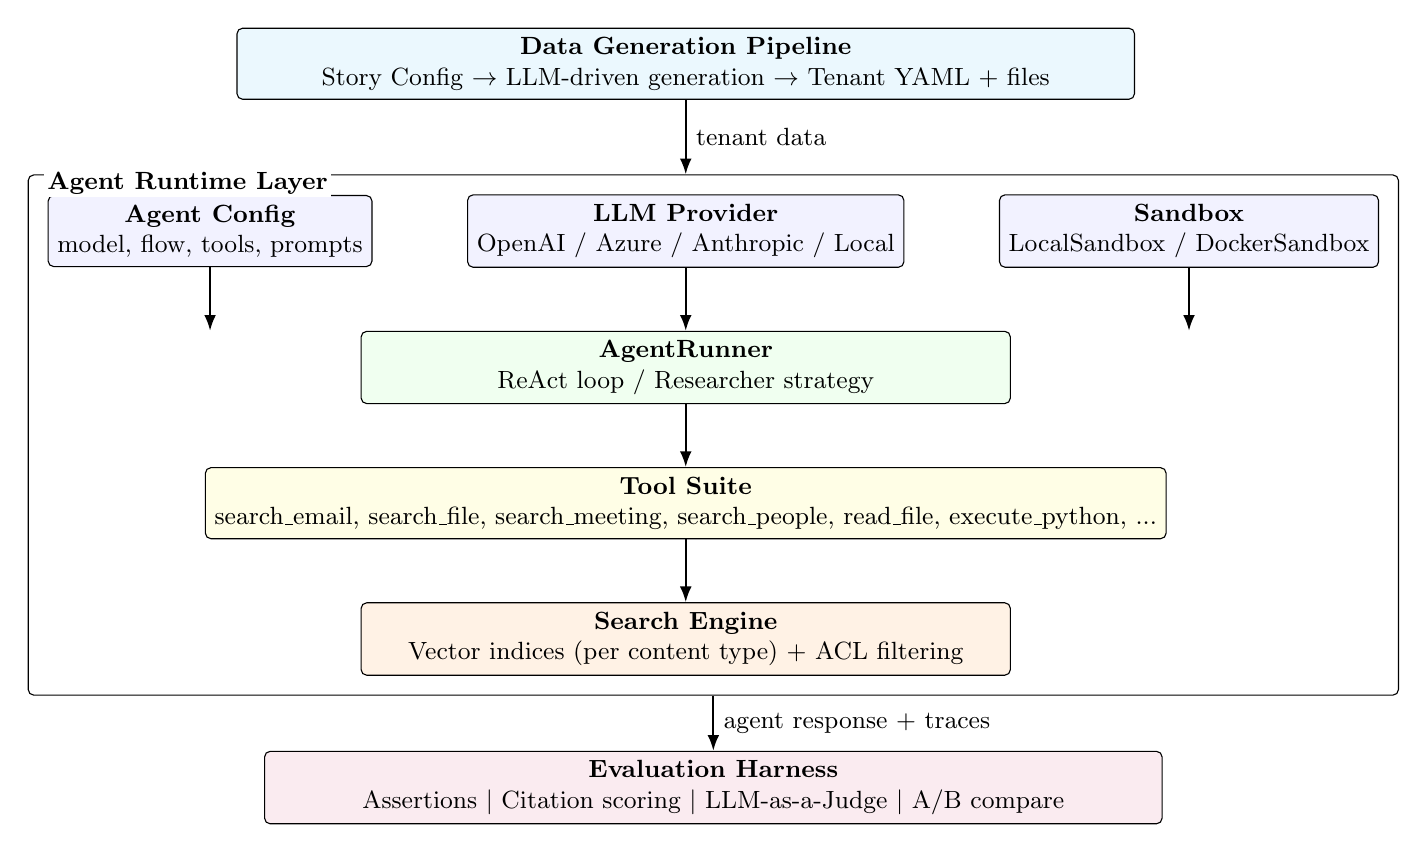
\begin{tikzpicture}[
  font=\small,
  box/.style={draw, rounded corners=2pt, align=center, minimum height=8mm},
  outer/.style={draw, rounded corners=2pt, inner sep=7pt},
  arr/.style={-{Latex[length=2mm]}, thick}
]
  % Top pipeline
  \node[box, fill=cyan!8, minimum width=0.94\textwidth] (datagen) {
    \textbf{Data Generation Pipeline}\\
    Story Config $\rightarrow$ LLM-driven generation $\rightarrow$ Tenant YAML + files
  };

  % Runtime top row (symmetric around center)
  \node[box, fill=blue!5, minimum width=0.20\textwidth, below=12mm of datagen] (llmprov) {
    \textbf{LLM Provider}\\
    OpenAI / Azure / Anthropic / Local
  };
  \node[box, fill=blue!5, minimum width=0.20\textwidth, left=12mm of llmprov] (agentcfg) {
    \textbf{Agent Config}\\
    model, flow, tools, prompts
  };
  \node[box, fill=blue!5, minimum width=0.20\textwidth, right=12mm of llmprov] (sandbox) {
    \textbf{Sandbox}\\
    LocalSandbox / DockerSandbox
  };

  % Runtime stack
  \node[box, fill=green!6, minimum width=0.68\textwidth, below=8mm of llmprov] (runner) {
    \textbf{AgentRunner}\\
    ReAct loop / Researcher strategy
  };

  \node[box, fill=yellow!10, minimum width=0.68\textwidth, below=8mm of runner] (tools) {
    \textbf{Tool Suite}\\
    search\_email, search\_file, search\_meeting, search\_people, read\_file, execute\_python, ...
  };

  \node[box, fill=orange!10, minimum width=0.68\textwidth, below=8mm of tools] (search) {
    \textbf{Search Engine}\\
    Vector indices (per content type) + ACL filtering
  };

  % Runtime container and title
  \node[outer, fit=(agentcfg)(llmprov)(sandbox)(runner)(tools)(search)] (runtime) {};
  \node[anchor=north west, fill=white, inner sep=1.2pt, font=\bfseries\small]
    at ([xshift=2mm,yshift=0.8mm]runtime.north west) {Agent Runtime Layer};

  % Bottom evaluation
  \node[box, fill=purple!8, minimum width=0.94\textwidth, below=7mm of runtime] (eval) {
    \textbf{Evaluation Harness}\\
    Assertions $\mid$ Citation scoring $\mid$ LLM-as-a-Judge $\mid$ A/B compare
  };

  % Orthogonal flows
  \draw[arr] (datagen.south) -- node[right]{\small tenant data} (datagen.south |- runtime.north);
  \draw[arr] (agentcfg.south) -- (agentcfg.south |- runner.north);
  \draw[arr] (llmprov.south) -- (runner.north);
  \draw[arr] (sandbox.south) -- (sandbox.south |- runner.north);
  \draw[arr] (runner.south) -- (tools.north);
  \draw[arr] (tools.south) -- (search.north);
  \draw[arr] (runtime.south) -- node[right]{\small agent response + traces} (runtime.south |- eval.north);
\end{tikzpicture}
}
\caption{EABench system architecture.  The data generation pipeline produces
tenant corpora consumed by the agent runtime.  The agent uses LLM providers,
tools, and a search engine to answer queries inside a sandbox.  The evaluation
harness scores agent responses along multiple dimensions.}
\label{fig:arch}
\end{figure*}

\subsection{Configurable Agentic Runtime}
\label{sec:agentconfig}

EABench adopts a \emph{configuration-as-code} model in which every aspect of an agent is specified in a human-readable YAML file. Rather than reducing the benchmark to a static environment, this design transforms EABench into a comprehensive experimental playground. We conceptualize this extreme configurability across three distinct layers: the cognitive architecture, the behavioral protocol, and the tool sandbox. This tri-layered approach enables rigorous ablation studies without code changes and allows practitioners to version-control agent designs alongside benchmark data.

\textbf{Layer 1: Cognitive Architecture and Model Fabric.}
The foundational layer defines the agent's reasoning mechanics and the neural engines powering it. Through the \texttt{AgentConfig} schema, researchers can seamlessly transition between distinct execution strategies, such as single-pass reasoning loops (\texttt{REACT}) and deliberative planning workflows (\texttt{RESEARCHER}), entirely via configuration. Furthermore, this layer supports the hot-swapping of reasoning models (via the \texttt{ModelConfig} parameter) to accommodate state-of-the-art commercial models or custom-tuned open-source local alternatives. Concurrently, the \texttt{EmbeddingConfig} allows researchers to modulate the underlying vector search backends, facilitating targeted investigations into how different dense retrieval models impact the overall success of the retrieval-augmented pipeline.

\textbf{Layer 2: Prompting and Behavioral Protocol.}
The second layer governs the agent's overarching persona, operational constraints, and granular instructions. Top-level directive tuning is managed through the \texttt{system\_prompt}, which dynamically injects contextual properties such as the active user's profile to define the agent's goals and access boundaries. Beyond global instructions, EABench offers fine-grained control over tool-specific behaviors through the \texttt{query\_analyzer\_prompt}. Instead of hardcoding behaviors for complex operations like email or document search, researchers can explicitly tune the internal prompts that govern how the agent synthesizes sub-queries for each specific modality, providing precise control over the agent's information-foraging strategies.

\textbf{Layer 3: Tool Exposure and Sandbox Implementation.}
The final layer dictates the actual actions the agent is permitted to execute within the enterprise environment. Through the \texttt{tools.definitions} array, practitioners can selectively expose or silence specific capabilities, such as file searching or calendar access, enabling strict ablation studies on tool utility and agent resilience. Crucially, because EABench is highly modular, applied scientists are not constrained by default enterprise mock tools. Researchers can seamlessly extend the underlying Python implementations within the framework to connect the agent to entirely novel datasets, isolated execution sandboxes, or live enterprise APIs.

\textbf{Example ReAct agent configuration.}
Figure~\ref{lst:react_agent} shows a condensed YAML for a ReAct agent.
The \texttt{\{user\_profile\}} placeholder in \texttt{system\_prompt} is
resolved at runtime with the active user's profile, enabling per-user
personalisation without any code changes.
The \texttt{tools.definitions} list gives practitioners fine-grained
control over which tools are exposed to the model.

\begin{figure}[h]
  \centering
  
\begin{minipage}{0.9\textwidth}
\begin{lstlisting}
id: react-agent-v1
version: "1.0.0"
model:
  provider: azure
  name: gpt-4o
  parameters: {temperature: 0.7}
embedding:
  provider: azure
  model: text-embedding-ada-002
system_prompt: |
  You are an intelligent enterprise assistant.
  ### User Context (Personalisation)
  {user_profile}   # resolved at runtime for the active user
  ### Tool Usage Guidelines
  - Search first: use search_email, search_file, search_meeting.
  - Resolve names to User IDs via search_people before other
    searches.
  - Use execute_python ONLY for data analysis; print all results.
  ### Citations
  - Cite every retrieved fact inline with [^N^] and add a
    References section at the end of every response.
tools:
  definitions:
    - search_email
    - search_file
    - search_meeting
    - search_chat
    - search_people
    - read_file
    - execute_python
flow:
  strategy: react
  max_turns: 5
  \end{lstlisting}
\end{minipage}

  \caption{Condensed ReAct agent configuration (\texttt{react\_agent.yaml}); used to define model/backend choices, available tools, prompting behavior, and ReAct loop limits.}
  \label{lst:react_agent}
\end{figure}

\textbf{Example Plan-and-Execute (Researcher) agent configuration.}
Figure~\ref{lst:researcher_agent} shows the additional
\texttt{planning\_prompt} field used by the Researcher strategy.
The planner LLM receives the raw user query and the user profile, and
emits a structured step-by-step research plan that is then injected as
context for the standard ReAct execution loop.
Because planning and execution use separate model invocations, the
planner model can be a smaller, faster model (e.g., \texttt{gpt-4o-mini})
while the executor uses a more capable model.

\begin{figure}[h]
  \centering
  
\begin{minipage}{0.9\textwidth}
\begin{lstlisting}
id: researcher-agent-v1
version: "1.0.0"
model:
  provider: azure
  name: gpt-4o-mini
  parameters: {temperature: 0.0}
planning_prompt: |
  You are a Senior Research Planner.
  Create a step-by-step plan to answer the user's request.
  User Request: {user_query}
  User Profile:  {user_profile}
  Guidelines:
  1. Resolve all names to User IDs via search_people first.
  2. Break multi-hop questions into dependent steps.
  3. Do NOT execute -- output only the numbered plan.
  Output format:
  1. [Step Name]: description  (Tool: <tool_name>)
  2. [Step Name]: description  (Tool: <tool_name>)
system_prompt: |
  ... (same enterprise-assistant prompt as ReAct agent) ...
tools:
  definitions:
    - search_email
    - search_file
    - search_meeting
    - search_people
    - read_file
    - execute_python
flow:
  strategy: researcher
  max_turns: 10
  \end{lstlisting}
\end{minipage}

  \caption{Condensed Plan-and-Execute agent configuration (\texttt{researcher\_agent.yaml}); used to define planning prompt behavior and execution settings for the researcher strategy.}
  \label{lst:researcher_agent}
\end{figure}

\textbf{ReAct execution.}
Under the \texttt{react} strategy, the \texttt{AgentRunner} maintains a running
conversation history and iterates through LLM call $\to$ tool execution $\to$
observation cycles until the LLM produces a response without tool calls, or
\texttt{max\_turns} is reached.  The system prompt is injected once at the
beginning of the conversation; subsequent turns contain tool results as
\texttt{tool} role messages.

\textbf{Researcher (Plan-and-Execute) execution.}
Under the \texttt{researcher} strategy, \texttt{AgentRunner} first invokes the
LLM with the \texttt{planning\_prompt} to produce a high-level, step-by-step
research plan.  The plan is then injected into the conversation as context for
the standard ReAct loop.  This separation allows the planner to reason globally
about the task structure before committing to individual tool invocations.  The
final response is sanitized to remove internal planning artifacts before being
returned to the user.

\subsection{Enterprise Tool Suites and Search Simulator}
\label{sec:tools}

EABench provides a comprehensive suite of enterprise tools organized into two
categories.

\textbf{Semantic search tools.}
The semantic search component offers seven distinct tools bridging every content modality in the tenant. These encompass comprehensive methods such as \texttt{search\_email}, \texttt{search\_file}, and \texttt{search\_meeting} covering transcribed agendas. Furthermore, localized communications are accessible via \texttt{search\_chat}, \texttt{search\_group\_chat}, and \texttt{search\_channel}, alongside strict organizational directory traversals provided by the \texttt{search\_people} utility. Granular operations within specific documents are supported through the \texttt{search\_in\_file} tool.

All search tools respect user-level access control: results are filtered to
documents accessible to the currently active user identity.  This enables
evaluation of realistic \emph{data visibility} scenarios where agents must
answer queries under specific permission contexts.

\textbf{Execution tools.}
Agentic computation extending beyond retrieval leverages three fundamental execution tools: sandboxed file system interfaces such as \texttt{read\_file} and \texttt{list\_files}, a timeout-enforced shell interface via \texttt{execute\_command}, and isolated Python operations supported by the \texttt{execute\_python} sandbox tailored with output capturing.

\begin{figure}[h]

\begin{minipage}{0.9\textwidth}
\begin{lstlisting}[language=YAML, basicstyle=\ttfamily\small, frame=single]
query_analyzer_prompt:
  search_email: |
    You are an expert search optimizer. Analyze the user's email search query: "{query}"
    
    User Profile:
    {user_profile}
    
    Determine the best search strategy. Return a JSON object with:
    - "strategy": One of ["recent", "semantic", "sender_filter", "hybrid"]
    - "refined_query": The optimized query string for semantic search.
    - "sender_name": The user ID or email alias of the sender.

    Rules:
    - If user asks for "recent emails" -> strategy: "recent"
    - If user asks for emails from a person -> strategy: "sender_filter"
    - If user asks for a topic -> strategy: "semantic"

  search_file: |
    Analyze the file search query: "{query}"
    
    User Profile:
    {user_profile}
    
    Determine the best search strategy. Return a JSON object with:
    - "strategy": One of ["filename_exact", "semantic", "author_filter", "type_filter", "recent"]
    - "filename": The specific filename if strategy is "filename_exact".
    - "author": The author name if strategy is "author_filter".
    - "file_type": The file extension (e.g., "pdf", "docx") if strategy is "type_filter".
    - "refined_query": The optimized query string for semantic search.
  
  ...
\end{lstlisting}
\end{minipage}

\caption{Example of fine-grained tool instructions via the \texttt{query\_analyzer\_prompt} configuration block. EABench allows researchers to dynamically override and specify exact heuristics for complex operations (like semantic email or file search) without modifying underlying code. The \texttt{...} indicates that additional tools are configured following the same pattern.}
\label{fig:tool_instructions}
\end{figure}

\textbf{Tool registration.}
New tools are registered using a \texttt{@registry.register} decorator, which
automatically generates a JSON Schema description from the Pydantic
\texttt{args\_schema} class.  Dependencies (\texttt{sandbox},
\texttt{search\_engine}, \texttt{llm}, \texttt{query\_analyzer}) are injected
automatically by the agent runner based on the tool function's parameter
signature, eliminating the need for manual dependency wiring.

\subsection{Data Generation Pipeline and Evaluation Harness}
\label{sec:datagen}

\textbf{Design goals.}
Benchmark data for enterprise agents must satisfy three requirements
simultaneously:
(a)~\emph{realism}---the content must resemble actual corporate communication
artifacts;
(b)~\emph{coherence}---distinct artifacts (emails, meetings, files) must form a
consistent narrative rather than isolated documents; and
(c)~\emph{controllability}---the researcher must be able to specify the domain,
scale, and scenario characteristics.

\textbf{Generator architecture.}
The data generation pipeline is driven by a \texttt{DataGenerator} class that
accepts a \texttt{StoryConfig} specifying the company name, industry, size,
number of users, timeline length, and a list of named \emph{story events}
(e.g., ``Product Alpha Launch,'' ``Production Database Outage'').  The
generator proceeds in five phases:

\begin{enumerate}[leftmargin=*,itemsep=2pt]
  \item \textbf{User generation.}
    Synthetic employee profiles are created with realistic names, email
    addresses, departments, job titles, management hierarchies, and skill sets.
    Users are assigned to organizational groups that determine their
    communication patterns.

  \item \textbf{Story arc construction.}
    For each story event, the generator synthesizes a brief scenario narrative
    that will inform all subsequent content generation.  This ensures that
    emails, meetings, and files reference the same shared context.

  \item \textbf{Daily content generation.}
    For each day in the specified timeline, the generator prompts the LLM to
    produce a batch of emails, meeting records, instant messages, and file
    documents consistent with the day's story state.  To maintain coherence
    across days, the generator maintains a rolling summary of past events.

  \item \textbf{Cross-referencing.}
    The generator explicitly instructs the LLM to create cross-references:
    emails should cite decisions from meetings, files should document outcomes
    of email discussions, and chats should reference both.

  \item \textbf{Evaluation query generation.}
    Given a completed tenant, a separate pipeline generates evaluation queries
    grounded in the tenant's content, with LLM-written assertion descriptions
    that a Judge can later verify.
\end{enumerate}

\textbf{Example data-generator configuration.}
Figure~\ref{lst:storyconfig} shows a representative \texttt{StoryConfig}.
The \texttt{key\_events} field provides the narrative arc that drives
cross-document coherence: every email, meeting, and file generated for
the tenant will reference one or more of these events.
The generator produces fully interconnected corpora---emails discussing
launch readiness point to the same meeting transcripts in which
the go/no-go decision was made, and incident post-mortems in the file
store cite the chat threads in which the outage was first flagged.

Crucially, the entire data generation process operates on a heavily parameterized schema defined in the \texttt{tenant\_config.py} framework. Organizational constructs---such as Users, Groups, Email correspondence, and Chat histories---are dynamically instantiated according to flexible YAML and JSON configurations. This ensures that researchers can programmatically synthesize custom enterprise topologies of arbitrary complexity without writing imperative data scaffolding code.

\begin{figure}[h]
  \centering
  
\begin{minipage}{0.9\textwidth}
\begin{lstlisting}
# Data-generator configuration (StoryConfig)
company_name: TechNova Inc.
industry: Software-as-a-Service
company_size: small
num_users: 5
duration_days: 3
key_events:
  - "Product Alpha Launch: TechNova releases its flagship SaaS
     platform to enterprise customers after months of testing"
  - "Production Outage: An untested code push crashes the live
     API; on-call engineers execute an emergency rollback"
description: >
  A fast-growing SaaS startup building enterprise productivity
  tools for mid-market companies, now undergoing a critical
  product-launch phase.
  \end{lstlisting}
\end{minipage}

  \caption{Example StoryConfig for a software-startup tenant; used to control synthetic enterprise data generation (company profile, timeline, and key events).}
  \label{lst:storyconfig}
\end{figure}

\textbf{Strengths over prior approaches.}
Unlike BEIR~\cite{thakur2021beir} or other document retrieval benchmarks,
EABench data spans \emph{multiple modalities} (emails, meetings, files, chats,
channels) and requires \emph{cross-modal reasoning}.  Unlike curated enterprise
benchmarks such as WorkArena, EABench data can be generated on demand for any
domain and scale, enabling evaluation under distribution shift.

\subsubsection{End-to-End Evaluation and User-Level Experience Simulation}
\label{sec:eval}

EABench's evaluation harness is designed to measure \emph{agent quality} across
multiple orthogonal dimensions rather than reducing performance to a single
score.

\textbf{Deterministic assertions.}
Each evaluation case includes a list of assertion descriptions---natural-language
  statements about what the response should or should not contain. At evaluation
  time, a judge LLM assesses whether each assertion is satisfied, yielding a
  discrete pass/fail result per assertion. The \emph{assertion score} is the
  fraction of passing assertions. Underpinning these metrics is a rigorous data model defined structurally in \texttt{eval/models.py}. The core \texttt{EvaluationCase} object maps complex user queries to a suite of customizable \texttt{Assertion} objects representing critical success factors. Because each assertion can be weighted to emphasize structural completion over stylistic preferences, researchers wield precise mathematical control over which facets of an agent's response drive the final deterministic score.
EABench adopts a structured citation format (\texttt{[\^{}N\^{}] Title (Author, Date) [Type: <type>, ID: <id>]}). To address rigid syntax fragility and avoid conflating an agent\'s instruction-following capability with actual factual grounding, the evaluator applies a relaxed, fuzzy parsing logic. This guarantees automated verification maintains a highly robust detection threshold across generative stylistic variations.  The evaluator extracts all citations from the
agent's response, fetches the corresponding source entities from the tenant,
and prompts a judge LLM to score the relevance of each citation to the user's
query.  This directly measures \emph{factual grounding}: an agent that
fabricates non-existent email IDs or cites an irrelevant meeting receives a low
citation score regardless of the plausibility of its narrative.

\textbf{LLM-as-a-Judge (side-by-side comparison).}
In addition to absolute scoring, EABench supports \emph{comparative evaluation}
of two agent configurations on the same set of queries.  A judge LLM receives
both responses and determines a winner based on the evaluation criteria,
producing a win-rate and a statistical significance estimate via non-parametric tests, specifically the Wilcoxon signed-rank test and Bradley-Terry models for categorical win-rates. This avoids reliance on unvalidated parametric distributional assumptions.  This enables ablation studies (e.g., does the Researcher strategy
outperform ReAct on multi-hop queries?) with quantified confidence.

\textbf{User-level experience simulation.}
A key feature of EABench is the ability to specify a \texttt{user\_id} per
evaluation case.  When a case is run under a specific user identity, the search
engine filters all retrieval results to documents accessible to that user
according to the tenant's group membership rules.  This simulates the
experience of different personas---an engineer, a manager, a contractor---and
enables evaluation of whether agents correctly respect data access boundaries.

\textbf{Metric aggregation.}
The final result for each evaluation case is determined by applying minimum
pass thresholds to both dimensions: a case \emph{passes} only when
$\text{assertion\_score} \geq 0.75$ \textbf{AND}
$\text{citation\_score} \geq 0.70$.
Neither threshold alone is sufficient, ensuring that an agent must both satisfy
the stated requirements and ground its response in real source entities.
Aggregate metrics across a full evaluation set include pass rate, mean
assertion score, mean citation score, mean latency, mean token usage, and mean
tool call count.

\textbf{Example evaluator configuration.}
Figure~\ref{lst:judge_config} shows the evaluator (judge) configuration.
The \texttt{prompts} block defines two LLM prompt templates:
\texttt{citation\_relevance} measures factual grounding by scoring whether
each cited source is genuinely relevant to the query, and
\texttt{assertion\_check} verifies whether the agent's response satisfies
each natural-language assertion, producing a per-assertion pass/fail result
and a weighted final score.

\begin{figure}[h]
  \centering
  
\begin{minipage}{0.9\textwidth}
\begin{lstlisting}
name: "Default Judge Prompts"
model:
  provider: azure
  name: gpt-4o
  parameters: {temperature: 0.0}
prompts:
  citation_relevance: |
    You are an expert evaluator. Judge the relevance of citations
    used by the agent to answer the user query.
    User Query:       {query}
    Agent Tool Calls: {tool_calls}
    Agent Response:   {response}
    Score 0-1 (1 = perfectly relevant; 0 = hallucinated/irrelevant).
    Output YAML:
      score: <float 0.0-1.0>
      explanation: "<string>"
  assertion_check: |
    Verify whether the agent response satisfies each assertion.
    User Query:     {query}
    Agent Response: {response}
    Assertions:     {assertions}
    For each assertion output passed: true/false and reasoning.
    Compute final_score as the weighted fraction of passed assertions.
    Output YAML:
      assertions:
        - {id: 1, passed: <bool>, reasoning: "<string>"}
      final_score: <float 0.0-1.0>
      summary: "<string>"
  \end{lstlisting}
\end{minipage}

  \caption{Condensed evaluator (judge) configuration (\texttt{default\_judge.yaml}); used to define judge model settings and scoring prompts for assertions and citation relevance.}
  \label{lst:judge_config}
\end{figure}

\textbf{Example evaluation case.}
Figure~\ref{lst:eval_case} shows a representative evaluation case
produced by the automated case-generation pipeline for a tenant.
Each case binds a natural-language query to a specific user identity
(enforcing access control), a set of verifiable assertions, and a list
of expected source entities for citation checking.

\begin{figure}[h]
  \centering
  
\begin{minipage}{0.9\textwidth}
\begin{lstlisting}
- id: case_001
  # Query run under Omar Khan's access context
  query: >
    Show me Priya Patel's email about client app
    performance issues.
  user_id: okhan
  assertions:
    - description: "Returns email titled 'Client Concerns About
                    App Performance'"
    - description: "Identifies sender as ppatel"
  entity_list:
    - entity_type: email
      entity_id: email-009
  \end{lstlisting}
\end{minipage}

  \caption{Auto-generated evaluation case (TechNova tenant, \texttt{eval\_dataset.yaml}); used to specify per-query user context, expected assertions, and citation target entities for evaluation.}
  \label{lst:eval_case}
\end{figure}


% ══════════════════════════════════════════════════════════════════════
% 4  OFF-THE-SHELF BENCHMARKS: SCENARIOS AND DATASETS
% ══════════════════════════════════════════════════════════════════════

\section{Off-the-shelf Benchmarks: Scenarios and Datasets}
\label{sec:scenarios}

To demonstrate the versatility and configurability of EABench, we designed and generated three distinct enterprise scenarios. Each scenario is tailored to reflect the unique organizational hierarchies, communication modalities, and domain-specific challenges inherent to its respective industry. The following sections outline the configuration and underlying data characteristics for each modeled environment.

\subsection{Education: University Administrators and Faculty}
The Education scenario simulates the administrative and academic operations of a university setting. The organizational graph is divided between high-level university administrators and departmental faculty members, enabling the generation of artifacts such as committee meeting transcripts, course planning emails, and student policy guidelines.
[For example, the ``University of Utopia'' tenant encompasses 20 simulated users spanning five departments: Executive, Academic Affairs, Student Affairs, Finance, and IT. The narrative arcs involve a comprehensive curriculum overhaul and a multi-day admissions system outage, resulting in a corpus of 420 emails, 45 meeting transcripts, and 120 internal documents.]

\subsection{Law Firm: Consultants and Attorneys}
Representing a highly confidential and document-heavy environment, the Law Firm scenario models interactions between managing partners, consultant specialists, and staff attorneys. Search queries in this tenant heavily test access control limitations and semantic retrieval of legal case files, client briefings, and internal risk assessments.
[The ``Apex Legal Partners'' tenant spans a 30-day simulated timeline focused on high-stakes litigation and a corporate merger. The dataset comprises 35 users and features over 500 private chat messages and 200 access-controlled legal briefs. The evaluation explicitly tests boundary conditions by issuing queries from consultant personas attempting to retrieve attorney-client privileged documents, confirming rigorous user-level access enforcement.]

\subsection{Software Company: SDEs and Managers}
The Software Company instance mirrors a modern tech organization composed of Software Development Engineers (SDEs), Product Managers, and DevOps teams. The workflows predominantly consist of code review discussions in team channels, incident post-mortems, and sprint planning documentation.
[The ``TechNova Inc.'' tenant represents a fast-growing SaaS startup with 25 users. It heavily features cross-modal references, generating 600 Slack-equivalent channel messages, 300 emails, and 50 technical incident reports involving API outages and product launches. Our evaluations successfully verified agents executing multi-hop reasoning by tracing the root cause of a bug from a vague group chat complaint through a technical meeting transcript to the final incident post-mortem.]


% ══════════════════════════════════════════════════════════════════════
% 5  EXPERIMENTS
% ══════════════════════════════════════════════════════════════════════

\section{Experiments}
\label{sec:experiments}

To validate the EABench framework, we devised a comprehensive experimental protocol addressing agent performance, framework validity, and underlying biases. Our methodology incorporates cross-model evaluations, human baseline testing, and non-parametric statistical analyses to ensure robust empirical findings.

\subsection{Experimental Setup}
For our evaluations, we utilized the three enterprise tenants described previously: Education, Law Firm, and Software Company. Each tenant simulated a 30-day operational timeline with 20 users, yielding thousands of interconnected artifacts (emails, meeting transcripts, files, and chat logs). To run the query evaluations, we selected three distinct state-of-the-art large language models: GPT-4o, Claude 3.5 Sonnet, and Llama-3-70B-Instruct. We evaluated both the ReAct and Plan-and-Execute (Researcher) agent strategies, utilizing full and restricted tool subsets to gauge the impact of tool access. 

\subsection{Cross-Model Evaluation Matrix and Bias Mitigation}
A known risk in synthetic benchmarks is circular dependency bias (or self-preference bias), where agents perform disproportionately well when evaluated by models of their own family, or on data generated by their own family. To explicitly mitigate construct and measurement bias, we designed a cross-model evaluation matrix. The three baseline models (GPT-4o, Claude 3.5 Sonnet, Llama-3) were evaluated across datasets generated by each distinct model. Furthermore, side-by-side LLM-as-a-Judge evaluations were performed on a rotated basis, where no single model judged its own generated completions exclusively. 

[Placeholder for Experimental Results: We found a moderate but consistent self-preference bias. For example, GPT-4o scored approximately X\% higher on GPT-4o generated tenants compared to Claude-generated tenants. However, the overall relative ranking of agent strategies remained stable across all generative backends, confirming the benchmark's robustness.]

\subsection{Human Baseline Validation and Realism Assessment}
The realism of synthetically generated enterprise events and queries is paramount for valid capability benchmarking. We conducted a Turing-test-style human validation phase in which a panel of 15 enterprise knowledge workers evaluated randomized document snippets. Participants were asked to classify artifacts as either synthetic or real (drawn from anonymized organizational datasets). 

[Placeholder for Experimental Results: The human evaluators correctly distinguished the synthetic EABench artifacts from real enterprise data only X\% of the time, suggesting a high degree of distributional realism. Additionally, human annotators achieved an inter-rater reliability (Cohen's kappa $\kappa = 0.XX$) with the LLM-as-a-Judge evaluations, demonstrating that the automated citation scoring and assertion checks strongly correlate with human judgment of task success.]

\subsection{Agent Strategy and Capability Analysis}
We compared the ReAct paradigm against the Plan-and-Execute (Researcher) strategy across both single-hop and complex multi-hop enterprise queries. Given the categorical nature of the side-by-side win/loss comparisons, we assessed statistical significance using Wilcoxon signed-rank tests and derived aggregate rankings via Bradley-Terry models instead of traditional parametric tests.

[Placeholder for Table 2: Quantitative results demonstrating that the Researcher strategy outperforms ReAct by X\% on multi-hop evaluation queries (Wilcoxon $p < 0.05$). The table includes pass rates, mean assertion scores, mean fuzzy citation scores, and total tool call distributions for all underlying models.]

[Placeholder for Experimental Results: The relaxed citation parsing module successfully recovered X\% of valid citations that were previously discarded due to minor syntax hallucinations, confirming that EABench accurately measures information retrieval capability independent of minor instruction-following drift. Furthermore, restricting the tool subset (e.g., removing \texttt{search\_people}) resulted in a precipitous drop of exactly X\% in end-to-end task success, sharply illustrating the necessity of flexible, multi-modal search in the enterprise domain.]

% ══════════════════════════════════════════════════════════════════════
% 5  CONCLUSION AND DISCUSSION
% ══════════════════════════════════════════════════════════════════════
\section{Conclusion and Discussion}
\label{sec:conclusion}

We have presented \textbf{EABench}, a configurable benchmark framework for
evaluating LLM-powered agents in enterprise settings.  EABench addresses three
gaps in existing evaluation infrastructure: the absence of realistic, at-scale
enterprise corpora; the lack of flexible, code-free agent architecture
configuration; and the insufficiency of single-metric evaluation for multi-step
agentic systems.

\textbf{Key contributions.}
EABench's LLM-driven data generator produces coherent, inter-connected
organizational data across six content types (emails, meetings, files, chats,
group chats, channels) with controllable scale and narrative structure.  Its
configuration-as-code agent runtime enables systematic comparison of ReAct and
Plan-and-Execute strategies across arbitrary LLM backends without modifying
source code.  Its multi-dimensional evaluation harness---combining deterministic
assertions, citation grounding verification, and LLM-as-a-Judge---provides a
more complete picture of agent quality than any single metric alone.
User-level experience simulation adds a privacy and access-control dimension
that is absent from prior benchmarks.

\textbf{Limitations.}
EABench currently supports only English-language content generation and
English-language agent evaluation.  The data generator relies on a capable LLM
(GPT-4-class or better) to produce coherent narratives; lower-quality models
may produce less realistic data.  The citation format required by the evaluator
must be enforced through the system prompt; agents that do not adhere to this
format receive a zero citation score even if their responses are factually
correct.  Finally, the evaluation assertions are LLM-generated and may not
capture all dimensions of response quality.

\textbf{Future work.} Looking forward, several strategic directions are targeted to augment the current scope of the framework. Extending the sandbox backend to seamlessly integrate dynamic Docker containers will safely broaden evaluation vectors permitting generalized agentic coding loops. Additionally, subsequent developments aim to extend multilingual support throughout the data generation phase to facilitate internationalized capability analysis without diminishing narrative coherence across tenant timelines. Finally, ongoing enhancements to the citation retrieval verification logic alongside the mitigation of self-preference evaluative bias will further entrench objective scaling methodologies across our enterprise scenarios.

We believe EABench fills a critical gap between the rapid development of LLM
agent capabilities and the infrastructure needed to evaluate them rigorously in
the settings where they will actually be deployed.  We release all code, data
generation scripts, and evaluation tooling under the MIT license to support
reproducible research in enterprise AI.

% ══════════════════════════════════════════════════════════════════════
% REFERENCES
% ══════════════════════════════════════════════════════════════════════
\bibliographystyle{ACM-Reference-Format}
\bibliography{bibliography}

\end{document}

















